\section{Theoretical Background}\label{body_theoretical_background}
This chapter serves as a reference for the theoretical background necessary to understand the insights gained in the following experimental chapters.
Section \ref{theoretical_classification} discusses classification models used to train on the extended dataset resulting from the generative augmentation process. In it, \textit{Neural Networks} (NNs) for image classification are introduced and the baselines for later comparisons are examined.
Sections \ref{theoretical_da} and \ref{theoretical_gda} establish the foundation for data augmentation and generative data augmentation.
Following sections \ref{theoretical_gan}, \ref{theoretical_dcgan}, \ref{theoretical_cgan}, and \ref{theoretical_madgan} provide theoretical knowledge necessary to understand the GAN architectures and their differences. The narrative follows their increasing complexity, starting from vanilla GANs, moving through deep convolutional GANs and conditional GANs, before diving into the background of multi-agent diverse GANs.
The final section (\ref{theoretical_image_scores}) explains the theory behind the Inception Score and Fréchet Inception Distance, concluding with an examination of the state-of-the-art \textit{InceptionV3} model used to compute them.
% ########################################################################################################
% # START: IMAGE CLASSIFICATION MODELS
% ########################################################################################################
\subsection{Image Classification Models}\label{theoretical_classification}
\subsubsection{Neural Networks for Classification}
Convolutional Neural Networks (CNNs) have become the dominant architecture for image classification tasks due to their inherent ability to automatically learn hierarchical features from raw pixel data. At their core, CNNs are build up by a sequence of convolutional-, pooling- and fully connected layers to extract hierarchical features, and funneling the information, typically into the \(N\) classes defined by the training data. That is, in case of classification tasks. 

Convolutional layers employ learnable filters to detect local patterns in the two-dimensional information. The two-dimensionality is inherent to image data. Pooling layers reduce the spatial dimensions, translating incoming data to a lower-dimensional space. Fully connected layers then map the extracted information into class probabilities, utilizing the \textit{Softmax} activation function. The afore mentioned layers are discussed in greater detail, in the following subsections.

\vspace{1em}

\textbf{Convolutional Layers}\label{theoretical_classification_conv_layers}
These layers compute the output from the local regions of the input. Let $(r \times c)$ be the two-dimensional input, e.g., a grayscale image, where $r$ represents the number of rows and $c$ the number of columns. Thus, $r \cdot c$ denotes the size of the image. Furthermore, let $(a \times b)$ be a filter with kernel size $a \cdot b$, where the filter is smaller than the input. This filter is moved from the top-left to the bottom-right over the input.

In each iteration, the dot product between the respective coefficients of the input region and the coefficients of the filter is computed. The product determines how much of the feature is present. The result of the dot product is then processed by the activation function $g$, which applies a non-linear transformation to it. If the activation function is ReLU, for example, only positive values are retained, meaning negative responses are set to zero. The result serve as an input to the subsequent layer.

The stride determines how far the filter moves after each operation. For a stride of $s = 1$, the filter can be placed in $(r - a + 1)$ positions along the height and $(c - b + 1)$ positions along the width, leading to an output size of $(r - a + 1) \times (c - b + 1)$. In general, the output size in the two-dimensional case is given by:
\[
\lfloor\left( \frac{r - a + s}{s} \right) \times \left( \frac{c - b + s}{s} \right)\rfloor
\]
where $\lfloor \cdot \rfloor$ denotes the floor function, which ensures that the output size is an integer.An image of this process can be found in Figure \ref{fig:maucher_convolutional_filtering}, in the Appendix. This image shows an input of size $[10 \times 10]$ and a filter of size $[3 \times 3]$. With a stride of $s = 1$, the resulting layer has a size of $[8 \times 8]$ (computed as $\left(10 - 3 + 1\right) \times \left(10 - 3 + 1\right)$). 

The stride of the filter can also be greater than $1$. Additionally, there is the option to apply padding to the image. There are different ways to implement padding. When padding of size $p$ is applied, the output size for a square input and filter is calculated as follows:
\[
\textbf{Output size} = \left\lfloor \frac{r - a + 2p}{s} \right\rfloor + 1
\]
A well known source for the context of convolutional arithmetic is the paper \textit{A guide to convolutional arithmetic for deep learning}, by Dumoulin et al. 2018 \cite{Dumoulin2016TransposedConv}. Convolutional layers are highly versatile due to their ability to process arbitrary numbers of input and output channels, enabling their widespread application across domains such as image processing, signal analysis, and natural language understanding.

\vspace{1em}

\textbf{Pooling Layers}\label{theoretical_classification_pooling_layers}
A pooling layer reduces the spatial dimensions (height and width) of feature maps, effectively compressing data while preserving the number of channels. Similar to convolutional layers, pooling layers apply a filter operations, that moves by a given stride. Instead of summing elements covered by the filter, typically, the filter applies one of the following operations: Max-, Average-, Global Max- or Global Average Pooling. \footnote{Other types of pooling involve e.g., L2-norm-, stochastic- or learnable pooling. However, these are less common than the afore mentioned types.}

To give an example, starting with an input of size $[32 \times 32 \times 10]$, applying a pooling operation with a $[2 \times 2]$ filter and a stride of 2 results in an output size of $[16 \times 16 \times 10]$. This operation reduces the spatial dimensions by half while keeping the depth unchanged.

\vspace{1em}

\textbf{Fully-Connected Layers}\label{theoretical_classification_fully_connected_layers}
Fully-Connected (FC), also called \textit{Dense} layer, typically computes the scores for the respective classes. In the case of ten classes, the result is a volume of size $[1 \times 1 \times 10]$\footnote{Typically, the output from the layer before the FC one is \textit{flattened} into a one-dimensional vector, preserving all information but removing spatial structure. For example, a $[2 \times 2]$ layer would result in a vector of size $[1 \times 4]$.}. By this stage, all spatial information has been transformed, leaving a quasi-one-dimensional vector. 

In a fully connected (FC) layer, each input is connected to each output, meaning every neuron in the previous layer is linked to every neuron in the FC layer. The output is computed as the weighted sum of all inputs, followed by an activation function, leading to the final classification scores that represent the likelihood of the input belonging to each class. It is not unusual to stack FC layers progressively to refine these scores. The spatial dimensions are collapsed into a single vector of class scores, which are then used for classification. The class probabilities are obtained by applying the Soft-Max Function \ref{theoretical_activations_softmax}.

\textbf{Batch Normalization Layers}\label{theoretical_classification_batchnorm_layers}
With their introduction in \textit{Batch Normalization: Accelerating Deep Network Training by Reducing Internal Covariate Shift} by Ioffe et al. \cite{ioffe2015batchnormalizationacceleratingdeep}, Batch Normalization (batchnorm) established as an integral part of convolutional networks and neural networks in general. This type of layer normalizes its inputs to subsequent layers and thereby stabilizing the distribution of activations throughout the training process. This reduces the internal covariate shift, allowing for higher learning rates and faster convergence. By normalizing activations, batchnorm helps prevent gradients from vanishing or exploding. However, it does not prevent it entirely. Additionally, it can provide regularization benefits and eliminate the need for Dropout, in some cases. With the afore mentioned benefits, batchnorm layers are particularly beneficial for deep learning networks with many layers.


\textbf{Typical Activation Functions in CNNs}

\begin{itemize}
    \item \textbf{ReLU (Rectified Linear Unit)}: \label{theoretical_activations_relu}
    \begin{equation}
    g(x) = \max(0, x)
    \end{equation}
    ReLU is the most widely used activation function in CNNs. It introduces non-linearity while maintaining efficiency by outputting zero for negative values and passing positive values unchanged.

    \item \textbf{Leaky ReLU}: \label{theoretical_activations_leakyrelu}
    \begin{equation}
        f(x) =
        \begin{cases}
        0 \quad \text{if } x < 0 \\
        x \quad \text{otherwise}
        \end{cases}
    \end{equation}
    A variant of ReLU, Leaky ReLU allows small negative values to flow through, addressing the \textit{dying ReLU} problem where neurons can become inactive \cite{Lu_Lu_2020}. 

    \item \textbf{Sigmoid (Logistic)}:  \label{theoretical_activations_sigmoid}
    \begin{equation}
        g(x) = \frac{1}{1 + e^{-x}}
    \end{equation}
    The sigmoid function squashes values between 0 and 1, commonly used for binary classification tasks. However, it can suffer from vanishing gradients for very large or small inputs.

    \item \textbf{Tanh (Hyperbolic Tangent)}:  \label{theoretical_activations_tanh}
    \begin{equation}
        g(x) = \frac{2}{1 + e^{-2x}} - 1
    \end{equation}
    Tanh outputs values between -1 and 1 and is similar to the sigmoid, but with a wider output range, making it more effective in many scenarios compared to sigmoid.

    \item \textbf{Softmax}: \label{theoretical_activations_softmax}
    \begin{equation}
        g(x_i) = \frac{e^{x_i}}{\sum_{j} e^{x_j}}
    \end{equation}
    Softmax is typically used in the output layer of CNNs for multi-class classification. It converts logits into probabilities, ensuring that the sum of the outputs is 1.

    \item \textbf{Cross-Entropy Loss:} \label{theoretical_loss_crossentropy}
    \begin{equation}
        g(y, \hat{y}) = -\sum_{i} y_i \log(\hat{y}_i)
    \end{equation}
    Cross-entropy is a common loss function for classification tasks. It measures the dissimilarity between the true label distribution \( y \) and the predicted probability distribution \( \hat{y} \). Lower values indicate a better alignment between the predicted and true classes. For consistency, the cross-entropy function is denoted with \( g \) here, although it is more commonly represented in the literature as \( H(y, \hat{y}) \) or \( H(p, q) \), where \( p \) refers to the true label distribution and \( q \) to the output of the discriminative model.


\end{itemize}

\subsubsection{Classification Models for augmented Training}
The classification models, on which the data augmentation is tested, are simple CNN classifiers consisting of the described layers. A dedicated classifier architecture is created for each dataset: MNIST and Fashion-MNIST (\ref{used_datasets}). The main differences between these architectures is the number of blocks, made of two-dimensional \hyperref[theoretical_classification_conv_layers]{convolutional}, \hyperref[theoretical_classification_batchnorm_layers]{batchnorm} and \hyperref[theoretical_classification_pooling_layers]{pooling} layers. All models use the \hyperref[theoretical_activations_relu]{ReLU} function for activation of the convolutional layers and the \hyperref[theoretical_activations_softmax]{Softmax} function for the activation at their last dense layer, resulting in probability distribution over the space of classes. More on the specific model architectures and used metrics for evaluation can be found in chapter \ref{body_prelim}.

\subsubsection{Classification Model Performance Metrics} \label{theory_classification_performanc_metrics}
For the assessment of classification performance, several standard metrics are commonly used. \textit{Accuracy} gives a measure for the overall proportion of correctly predicted instances, but can be misleading in imbalanced datasets. \textit{Precision} quantifies the proportion of correctly predicted positive instances among all predicted instances, whereas \textit{recall} \footnote{Recall is also known as sensitivity.} captures the proportion of correctly predicted positives out of all actual positive samples. 

The \textit{F1 score} is the harmonic mean of precision and recall and serves as a balanced metric when both false positives and false negative are of concern. This is especially useful for imbalanced datasets. Mathematically, the formulation of the F1 score is as follows: 

\begin{equation}
    \mathrm{Precision} = \frac{TP}{TP + FP}, \quad \mathrm{Recall} = \frac{TP}{TP + FN}
\end{equation}

\begin{equation}
    \mathrm{F1} = 2 \cdot \frac{\mathrm{Precision} \cdot \mathrm{Recall}}{\mathrm{Precision} + \mathrm{Recall}}
\end{equation}    

Even when working with stratified data, where class distributions are balanced, the F1 score remains valuable by providing a single, informative measure that accounts for the trade-off between precision and recall. Due to its sensitivity to both types of classification errors, the F1 score is used as the primary evaluation metric throughout this work, in the context of classifications.

% ########################################################################################################
% # END: IMAGE CLASSIFICATION MODELS
% ########################################################################################################

% ########################################################################################################
% # START: DATA AUGMENTATION
% ########################################################################################################

\subsection[Data Augmentation - DA]{Data Augmentation}\label{theoretical_da}
In this chapter, data augmentation (DA) techniques in the context of images are discussed in greater detail, starting with traditional augmentations (e.g., rotating or cropping an image) and ending with generative augmentations, in which generative models are used to expand the training data of subsequent classification models.

\subsubsection[Traditional Data Augmentation - TDA]{Traditional Data Augmentation}\label{theoretical_tda}
The need for data augmentation to make classification algorithms more resilient has existed for decades. Early papers mentioning the augmentation of data for classification tasks date back to the 1960s \cite{Nagy1966} (1966). For the context of deep learning, however, the augmentation of images was popularized by Krizhevsky et al. in 2012 \cite{Krizhevsky2012traditionaldataaugmentation}. This paper introduced the \textit{AlexNet}, a deep CNN used to classify images from the \textit{ImageNet} dataset \cite{ImageNetDataset5206848}, containing $1 000$ classes. 

%This paper also referenced the earlier work of Simard et al. from 2003 \cite{Simard2003bestpracticesforcnns}.

Generally, traditional data augmentation (TDA) techniques can be described as applying transformations to the initial training data. These transformations preserve the respective labels \(y\) and only act on the data \(X\). \footnote{It is to point out, that there are also transformations to be applied to the labels. This can include operations like random flipping of the labels. Such alterations also include techniques such as smoothing the labels, e.g., adjusting labels to not be strictly $0$ or $1$, but rather $0.1$ or $0.9$.} Applied transformations could either be used to enlarge the training data or to alter existing data i.e., altering the variability in it.\\

Augmentations are categorized based on the type of transformations applied:

\begin{itemize}
    \item \textit{Geometric Augmentation}: This category modifies the shape, position, and perspective: Rotation, Scaling, Flipping, Cropping, Shearing, Perspective Transform.
    \item \textit{Photometric Augmentation}: Alters pixel values while keeping the spatial structure: Brightness, Contrast, Hue Shift, Blurring
    \item \textit{Noise-Corruption Augmentation}: Imitates real-world degradations and distortions caused by cameras and sensors: Gaussian Noise, Speckle Noise, Salt-and-Pepper Noise.
\end{itemize}

\noindent
Mathematically, let \( X \) be an original data sample drawn from the dataset distribution \( P(X) \). Traditional data augmentation applies a transformation function \( f: X \mapsto \tilde{X} \), where \( f \) is a function sampled from a predefined set of augmentation operations \( \mathcal{F} \). The augmented data sample \( \tilde{X} \) is then given by:

\[
\tilde{X} = f(X), \quad f \sim \mathcal{F}.
\]

\noindent
Since TDA modifies already existing samples, the distribution of augmented samples \( P_{\tilde{X}} \) should ideally remain close to the original data distribution:

\[
P_{\tilde{X}}(X) \approx P(X).
\]

\noindent
In the context of data augmentation pipelines, this can be generalized as:

\[
\text{TDA}: (X, f) \mapsto \tilde{X}, \quad f \in \mathcal{F}.
\]

\begin{figure}[htbp]
    \centering
    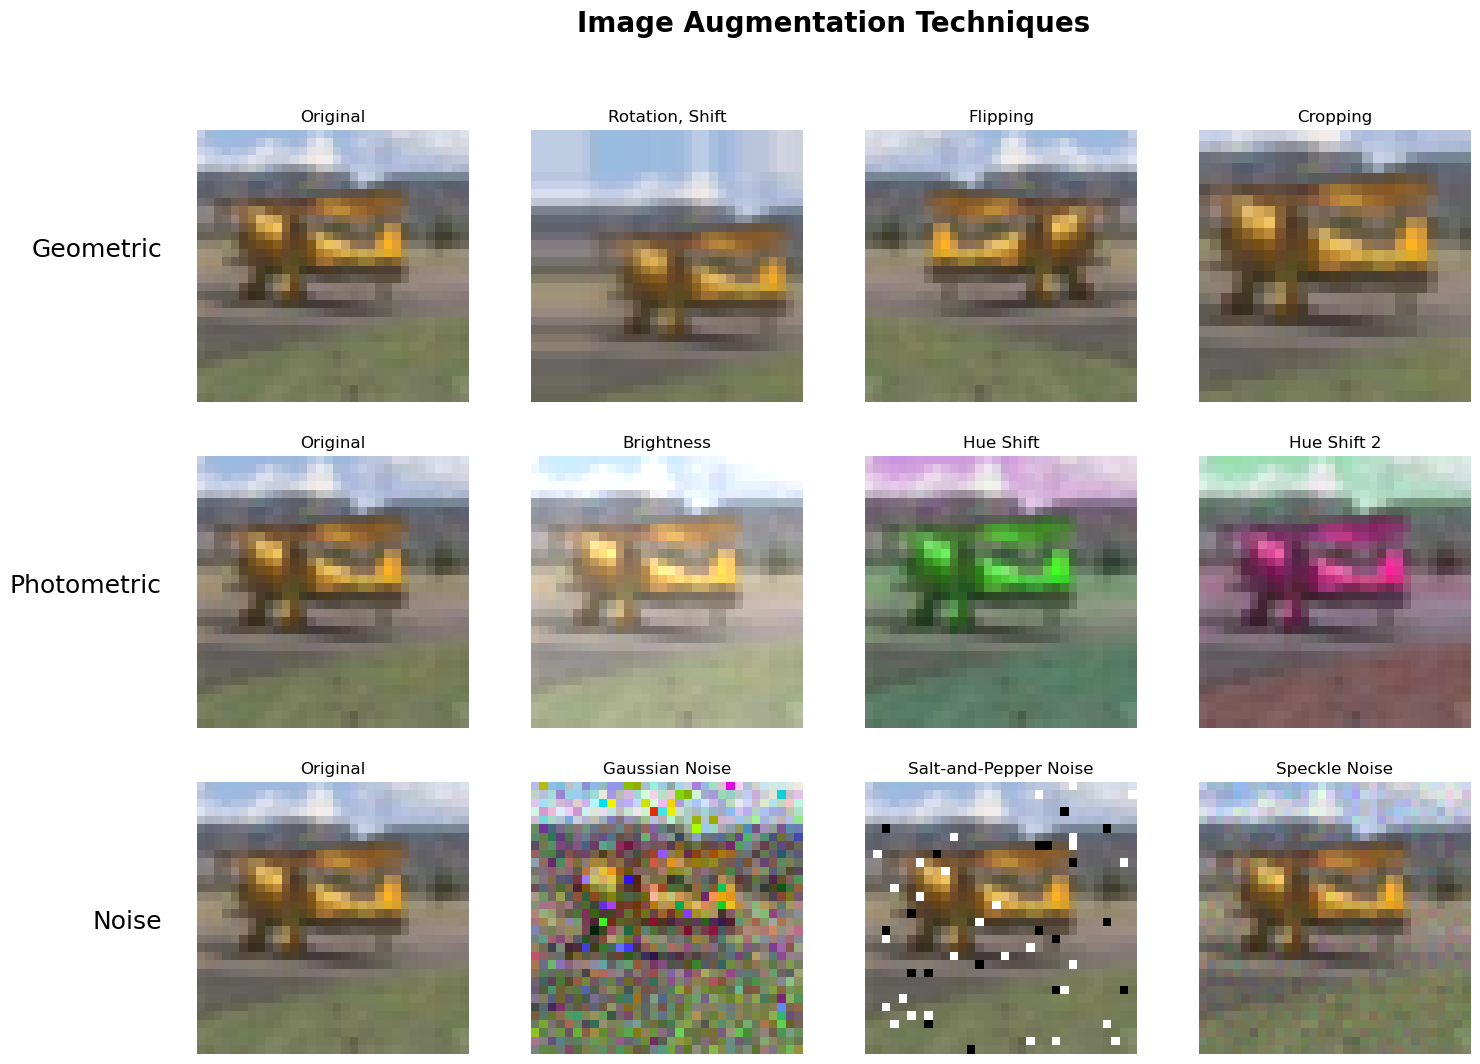
\includegraphics[width=.9\textwidth]{abb/traditional_image_augmentation_examples.png}
    \caption{Exemplary use of traditional augmentation techniques from the categories \textit{geometric} (first row), \textit{photometric} (second row), and \textit{noise-corruption} (third row). The image shown is an image from the \hyperref[used_datasets]{CIFAR10 dataset}, assigned to the class \textit{airplane}.}
    \label{fig:figure_tda_examples}
\end{figure}

\noindent
When applying the augmentations shown in Figure \ref{fig:figure_tda_examples}, it is mandatory to consider domain-specific knowledge and constraints. For example, flipping images from the MNIST dataset to train a generative model may result in an image where a horizontally flipped \textit{9} appears. This is in the domain of Arabic numerals semantically incorrect. Further, flipping a $9$ along horizontal and vertical axes would result in a $6$. Conversely, when classifying airplanes—which can vary in shape, color, three-dimensional orientation, and images may be taken through a dusty lens—applying most of the above augmentations could be beneficial, except for horizontal flipping, as mentioned above.


\subsubsection[Generative Data Augmentation - GDA]{Generative Data Augmentation}\label{theoretical_gda}
Differing from the previously mentioned TDA \ref{theoretical_tda}, generative data augmentation (GDA) techniques do not focus on altering existing data instances. Rather, it focuses on creating entirely new samples that match the underlying data distribution of the training data. These generated instances may or may not include labels.

The goal is to train a generative model \( G \) that produces instances \( X_1 \), for example, from a noise vector \( z \) \footnote{A noise vector may serve as input for a Generative Adversarial Network. See: \ref{theoretical_gan}}, such that the distribution of the generated data approximates the true distribution \( P(X) \) of the original dataset. In this context, \( G \) can be viewed as a function:

\[
G: z \mapsto X_1, \quad X_1 \sim P_G(X_{fake}) \approx P(X),
\]

\noindent
where \( P_G(X_{fake}) \) is the learned distribution of the generative model, aiming to approximate the real data distribution \( P(X) \).

In the case of \textit{conditional} generative data augmentation, additional information such as class labels \( y \) is incorporated into the generation process. This allows the model to generate samples corresponding to specific categories within the data. The conditional generative model \( G \) then follows:

\[
G: (z, y) \mapsto X_{fake}, \quad X_{fake} \sim P_G(X_{fake} \mid y) \approx P(X \mid y),
\]

\noindent
where \( P_G(X{fake} \mid y) \) represents the learned conditional distribution, aiming to approximate the real class-conditioned data distribution \( P(X \mid y) \). This can enable targeted data generation for specific categories, enhancing data diversity while maintaining class consistency.

% ########################################################################################################
% # END: DATA AUGMENTATION
% ########################################################################################################



% ########################################################################################################
% # START: Generative Aderserial Networks
% ########################################################################################################

\subsection[Generative Adversarial Network - GAN]{Generative Adversarial Network}\label{theoretical_gan}
Generative Adversarial Networks (GANs) have first been introduced by Goodfellow et al. in 2014 \cite{goodfellow2014generativeadversarialnetworks} GANs are a type of generative models designed to learn the underlying data distribution of their training data and generate new, realistic instances. The core idea of the framework is an adversarial training process between two neural networks (NNs): the \textit{Generator} \(G\) and \textit{Discriminator} \(D\), are competing against one another in a minimax game \cite{VonNeumann1928Minimax}. The following figure (\ref{fig:figure_gan_arch}) shows a visualization of the vanilla GAN architecture.

\begin{figure}[htbp]
    \centering
    \vspace{-4em}
    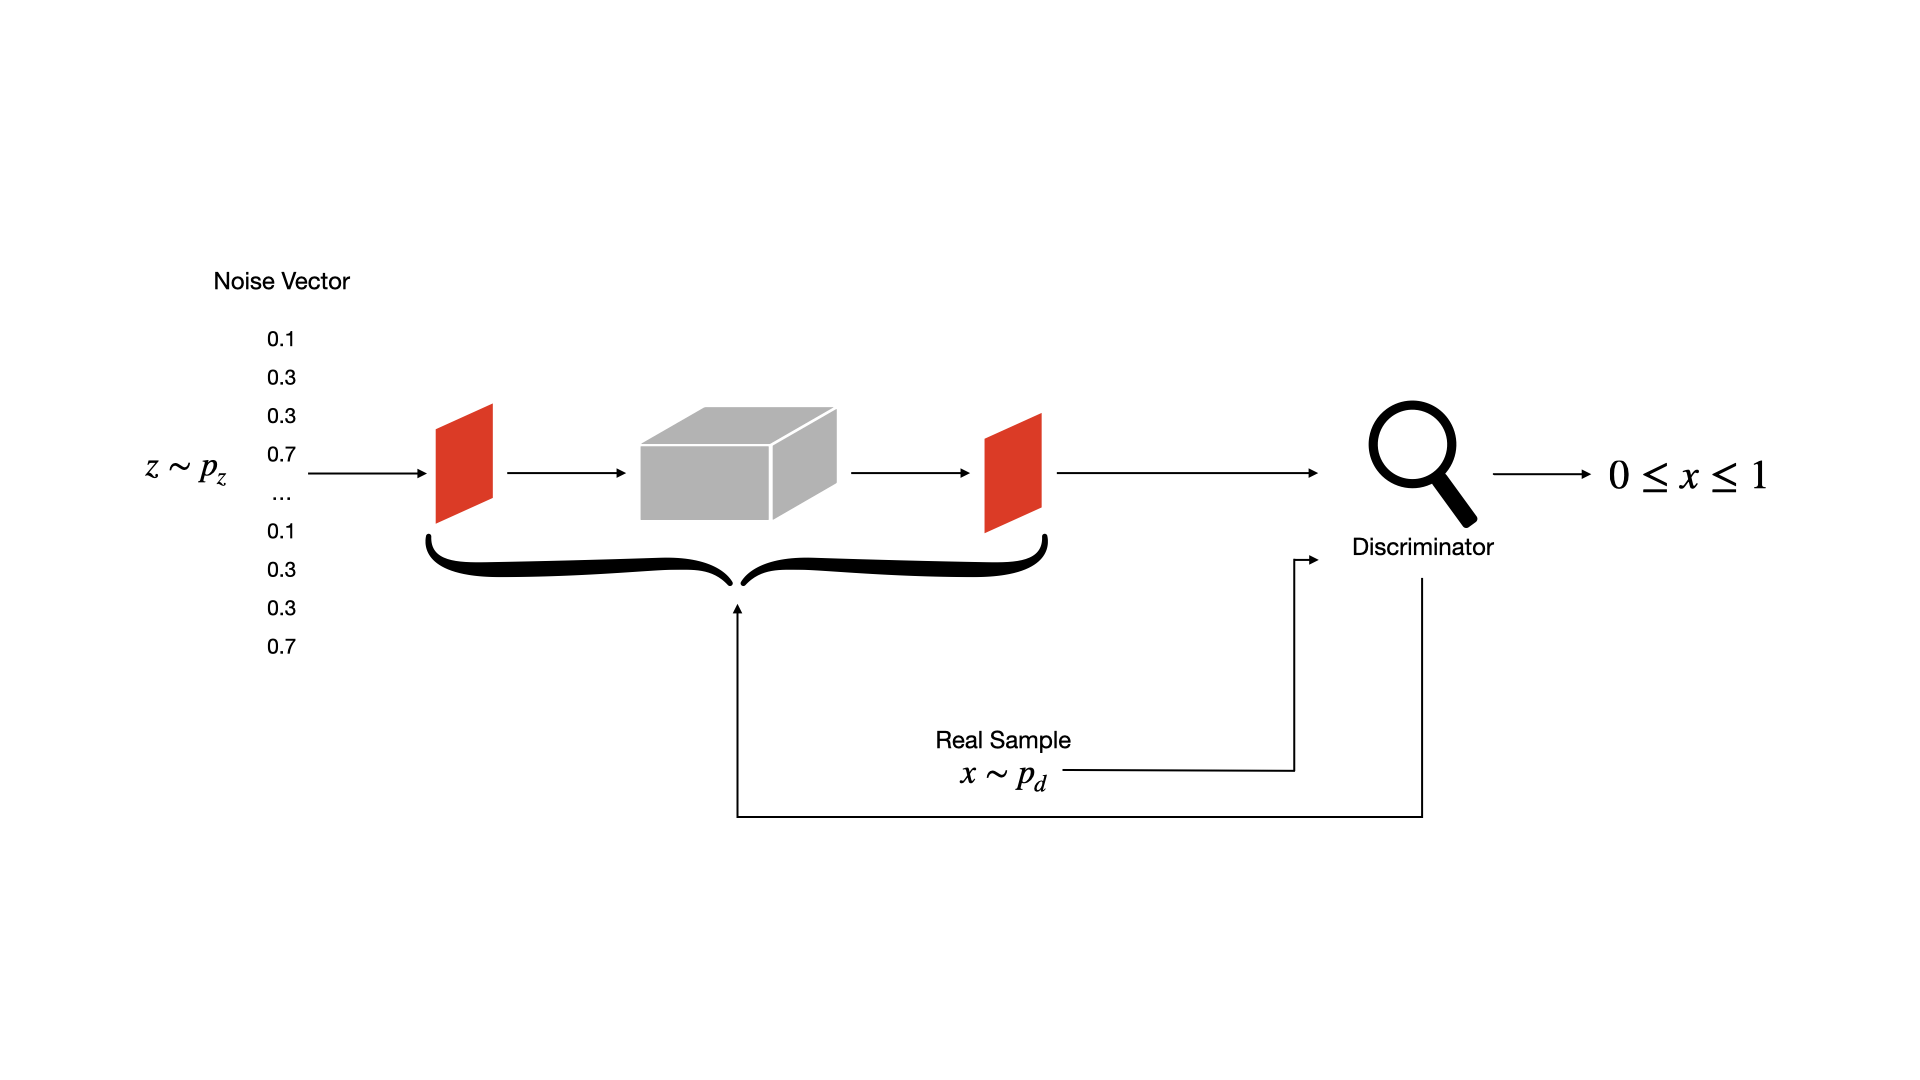
\includegraphics[width=.9\textwidth]{abb/arch_gan.png}
    \caption{Visualization of the vanilla GAN architecture. The figure shows the noise vector flowing into the generator. The generators output, as well as the real sample from \(P_{data}\), flow into the discriminator.}
    \label{fig:figure_gan_arch}
\end{figure}


\subsubsection{Mathematical Formulation}\label{theoretical_gan_math}
Let \(X \sim P_{data}\) be samples drawn from the real data distribution, and let \(z \sim P_z\) be random noise sampled from a known prior (e.g., a Gaussian or uniform distribution). The generator \(G\) is a function \(G(z): \mathbb{R}^{d_z} \to \mathbb{R}^{H \times W \times C}\), with \textit{H, W, C} as the height, width, and the number of channels, that maps a noise vector \(z\) to a synthetic data instance \(\tilde{X}\), attempting to approximate \(P_{data}\):\(\tilde{X} = G(z), \quad z \sim P_z.\)

The discriminator \(D\) is a function \(D: \mathbb{R}^{H \times W \times C} \to [0,1]\) that outputs the probability that a given sample is real or generated. It is trained to distinguish between real samples \(X \sim P_{data}\) and generated samples \(\tilde{X} \sim P_G\), where \(P_G\) is the implicit distribution induced by \(G\).

The training objective is formulated as the following minimax game:

    \begin{equation}\label{theory_gan_vanilla_formula}
        \mathcal{L}_{\text{adv}} = \min_G \max_D \mathbb{E}_{X \sim P_{data}} [\log D(X)] + \mathbb{E}_{z \sim P_z} [\log (1 - D(G(z)))].
    \end{equation}

Here, the discriminator \(D\) aims to maximize the probability of correctly identifying real samples \(D(X)\), with \(X \sim P_{data}\). The generator \(G\) aims to generate samples that fool \(D\), minimizing \(\log(1 - D(G(z)))\). In an ideal scenario, the game converges to a \textit{Nash equilibrium}, a concept from game theory. At this point, a stable state is reached where no player can benefit by unilaterally adjusting their strategy, assuming the other players keep their strategies unchanged. \(G\), in this case, produces samples indistinguishable from real data, i.e., \(P_G \approx P_{data}\). In this scenario, the discriminators output oscillates around $0.5$, continuously unable to differentiate real and fake samples.

\subsubsection{Training Process}\label{theoretical_gan_training}
GAN training follows an alternating optimization approach. Typically, alternating training the generator and the discriminator:
\begin{enumerate}
    \item Update \(D\): Given a batch of real samples from \(P_{data}\) and fake samples generated by \(G\), update \(D\) to maximize its ability to discriminate real from fake data.
    \item Update \(G\): Generate new fake samples and update \(G\) to minimize \\ \(\log(1 - D(G(z)))\), effectively pushing \(G\) to generate more realistic samples.
    \item Repeat the process iteratively, typically using stochastic gradient descent (SGD) or Adam optimization.
\end{enumerate}

\subsubsection{Challenges in GAN Training}\label{theory_gan_problems}
Next, challenges that can occur during the training of GANs are discussed. These have already been mentioned in the introductory section \ref{problems_of_gans}. Here, the afore mentioned challenges are described in detail.

\paragraph[Mode Collapse]{Mode Collapse}
Mode collapse occurs when the generator produces only a small subset of the data distribution, leading to a lack of diversity. Instead of generating varied diverse samples, it repeatedly produces similar ones that fool the discriminator. This happens when the generator finds an easy \textit{shortcut} rather than learning the full distribution over all classes. More formally, \(G\) collapses many values of \(z\) to the same value of \(x\) \cite{goodfellow2014generativeadversarialnetworks}. A common technique to mitigate this issue is minibatch discrimination \cite{salimans2016improvedtechniquestraininggans}. In several studies, experiments have been conducted to enhance diversity of GANs (\cite{Chang2024QDGenSampling}, \cite{Humayun2021MaGNET}, \cite{Humayun2022PolaritySampling}) % TODO: I tried minibatch discrimination for the cifar madgan, but did not work
\paragraph[Lack of Inter-Class Diversity]{Lack of Inter-Class Diversity}
Even if mode collapse is avoided, GANs may struggle to generate samples that represent all data classes equally. This is a common issue in class-conditional GANs, where samples across different classes may overlap or lack distinct features. Causes include imbalanced datasets, poor class conditioning, or weak discriminator feedback \cite{Odena201710.5555/3305890.3305954}.

\paragraph[Failure to Converge]{Failure to Converge}
Unlike traditional neural networks, GANs follow an adversarial training process, making optimization highly unstable. The loss functions of both the generator and discriminator change dynamically, often leading to non-convergent behavior. Methods like Wasserstein GANs (WGAN) \cite{arjovsky2017wassersteingan} and spectral normalization \cite{miyato2018spectralnormalizationgenerativeadversarial} improve stability and help achieve better convergence.

\paragraph[Vanishing & unstable Gradients]{Vanishing \& unstable Gradients}
When the discriminator becomes too strong, it perfectly distinguishes real from fake samples, leading to vanishing gradients for the generator. This prevents meaningful updates and stalling progress. On the other hand, unstable gradients cause erratic updates, preventing smooth learning. Alternative loss functions (e.g., LSGANs \cite{mao2017squaresgenerativeadversarialnetworks}) and spectral normalization can help stabilize the training.

\paragraph[Imbalance between Generator and Discriminator]{Imbalance between Generator and Discriminator}
A well-balanced GAN requires both models to improve at a similar pace. If the discriminator overpowers the generator, gradient updates to the generator can vanish. If it's too weak, the generator receives poor feedback and produces low-quality outputs \cite{goodfellow2014generativeadversarialnetworks}. Balancing techniques include adaptive learning rates, gradient penalties, and label smoothing \cite{Radford2015DCGAN}. Another interesting alternative, to tackle the problem of imbalance is introduced in the paper \textit{Progressive Growing of GANs for Improved Quality, Stability, and Variation} \cite{karras2018progressivegrowinggansimproved}.


\subsection[Deep Convolutional Generative Adversarial Network - DCGAN]{Deep Convolutional Generative Adversarial Network}\label{theoretical_dcgan}
Deep Convolutional Generative Adversarial Networks (DCGANs) were introduced by Radford et al. in 2015 \cite{Radford2015DCGAN} as an improvement over vanilla GANs. While the fundamental adversarial framework remains the same (see \hyperref[theoretical_gan_math]{3.3 Mathematical Formulation}, \hyperref[theoretical_gan_training]{3.3 Training Process}), DCGANs leverage deep convolutional neural networks to enhance stability and generate higher-quality images.

\subsubsection{Architectural Adjustments}\label{theorey_dcgan_architecture}
To improve training stability and image quality, DCGANs replace fully connected layers with convolutional layers, enabling enhanced spatial feature extraction. Following, the benefits of the layers for this context is briefly mentioned.

\begin{itemize}
    \item \textbf{Convolutional Architecture:} Fully connected layers in both \(G\) and \(D\) are replaced with deep convolutional layers, enabling better spatial feature extraction.
    \item \textbf{Strided Convolutions:} In the discriminator, pooling layers are removed in favor of strided convolutions, reducing the risk of information loss.
    \item \textbf{Transposed Convolutions:} The generator employs transposed convolutions (also known as fractionally-strided convolutions) instead of upsampling layers to improve the quality of generated images.
    \item \textbf{Batch Normalization:} Applied to both \(G\) and \(D\), batchnorm helps stabilize training by reducing internal covariate shift \ref{theoretical_classification_batchnorm_layers}. Batchnorm is omitted in the generators final layer to allow unrestricted output variability and in the discriminators input layer to preserve the original data distribution.
    \item \textbf{LeakyReLU Activation:} The discriminator uses LeakyReLU instead of standard ReLU to prevent dying neurons and allow gradients to flow through negative inputs \ref{theoretical_activations_leakyrelu}.
    \item \textbf{No Fully Connected Layers:} Fully connected layers are removed to maintain spatial coherence in generated images, as they discard spatial information by flattening feature maps. Instead, convolutional layers preserve local structures, enabling more realistic image synthesis \ref{theoretical_classification_fully_connected_layers}.
\end{itemize}


\subsection[Conditional Generative Adversarial Network - cGAN]{Conditional Generative Adversarial Network}\label{theoretical_cgan}

Conditional Generative Adversarial Networks (cGANs), introduced by Mirza and Osindero in 2014 \cite{mirza2014conditionalgenerativeadversarialnets}, extend the vanilla GAN framework by incorporating additional information \(y\), such as class labels, into both the generator and discriminator. This allows cGANs to generate samples conditioned on specific attributes, enabling controlled generation.

\subsubsection{Mathematical Formulation}
\label{theoretical_cgan_math}
The core idea of cGANs is to condition both the generator \(G\) and the discriminator \(D\) on auxiliary information \(y\). Instead of generating data solely from a noise vector \(z\), the generator now takes \(y\) as an additional input:

\begin{equation}
\tilde{X} = G(z, y)
\end{equation}

\noindent
Similarly, the discriminator receives both the real or generated sample and the corresponding condition:

\begin{equation}
D(X, y) \quad \text{and} \quad D(G(z, y), y)
\end{equation}

\noindent
The adversarial objective function for cGANs extends the standard GAN loss to incorporate this conditional dependency:

\begin{equation}\label{theory_gan_cond_formula}
\mathcal{L}_{\text{adv}} = \min_G \max_D \mathbb{E}_{X, y \sim P_{data}} [\log D(X, y)] + \mathbb{E}_{z \sim P_z, y \sim P_y} [\log (1 - D(G(z, y), y))]
\end{equation}

\noindent
This objective encourages the generator to produce samples that are not only realistic but also consistent with the provided condition, while the discriminator is trained to discern real from synthetic data based on their respective conditions.

\subsubsection{Architectural Adjustments}
\label{theory_cgan_architecture}
To implement cGANs, architectural adjustments are necessary compared to vanilla GANs:

\begin{itemize}
    \item \textbf{Input Conditioning:} Both the generator and discriminator must receive the conditional information \(y\) as input. This is typically achieved by concatenating the condition y with the noise vector z in the generator's input and with the input image \(X\) in the discriminators input.
    \item \textbf{Embedding Conditional Information:} For categorical conditions e.g., class labels, the condition \(y\) is often embedded into a lower-dimensional vector before concatenation. This embedding allows the network to learn meaningful representations of the conditions.
    \item \textbf{Concatenation, Addition, or Multiplication:} The conditional information can be incorporated through concatenation, addition, or element-wise multiplication at various layers within the generator and discriminator, depending on the specific application and architecture.
    \item \textbf{Preservation of Conditional Information:} Care must be taken, that the conditional information is preserved throughout the network. This means, that the information must traverse the network, all the way to the output layer.
\end{itemize}

\noindent
These architectural modifications ensure that the generator and discriminator can effectively utilize the conditional information to generate and discriminate samples based on the given conditions.

\subsection[Multi-Agent Diverse Generative Adversarial Network - MADGAN]{Multi-Agent Diverse Generative Adversarial Network}
\label{theoretical_madgan}
MADGAN is proposed as a generalized framework for the GAN architecture \cite{ghosh2018madgan}. The framework employs multiple generators, one discriminator and an adjusted objective for the discriminator. The adjusted objective aims to enforce the identifications of the generator creating given fake images \(G_{i} \hat{x}\). These changes specifically aim to ease the first two mentioned problems of GANs, namely \textit{Mode Collapse} and \textit{Lack of Inter-Class Diversity} \ref{theory_gan_problems}. This chapter delves into the specifics of this framework: integration of multi-agent systems with diversity-promoting techniques, within the GAN framework. The following subsections will detail the architecture, objective function, and training procedure of the MADGAN framework.

\begin{figure}[htbp]
    \centering
    \vspace{-4em}
    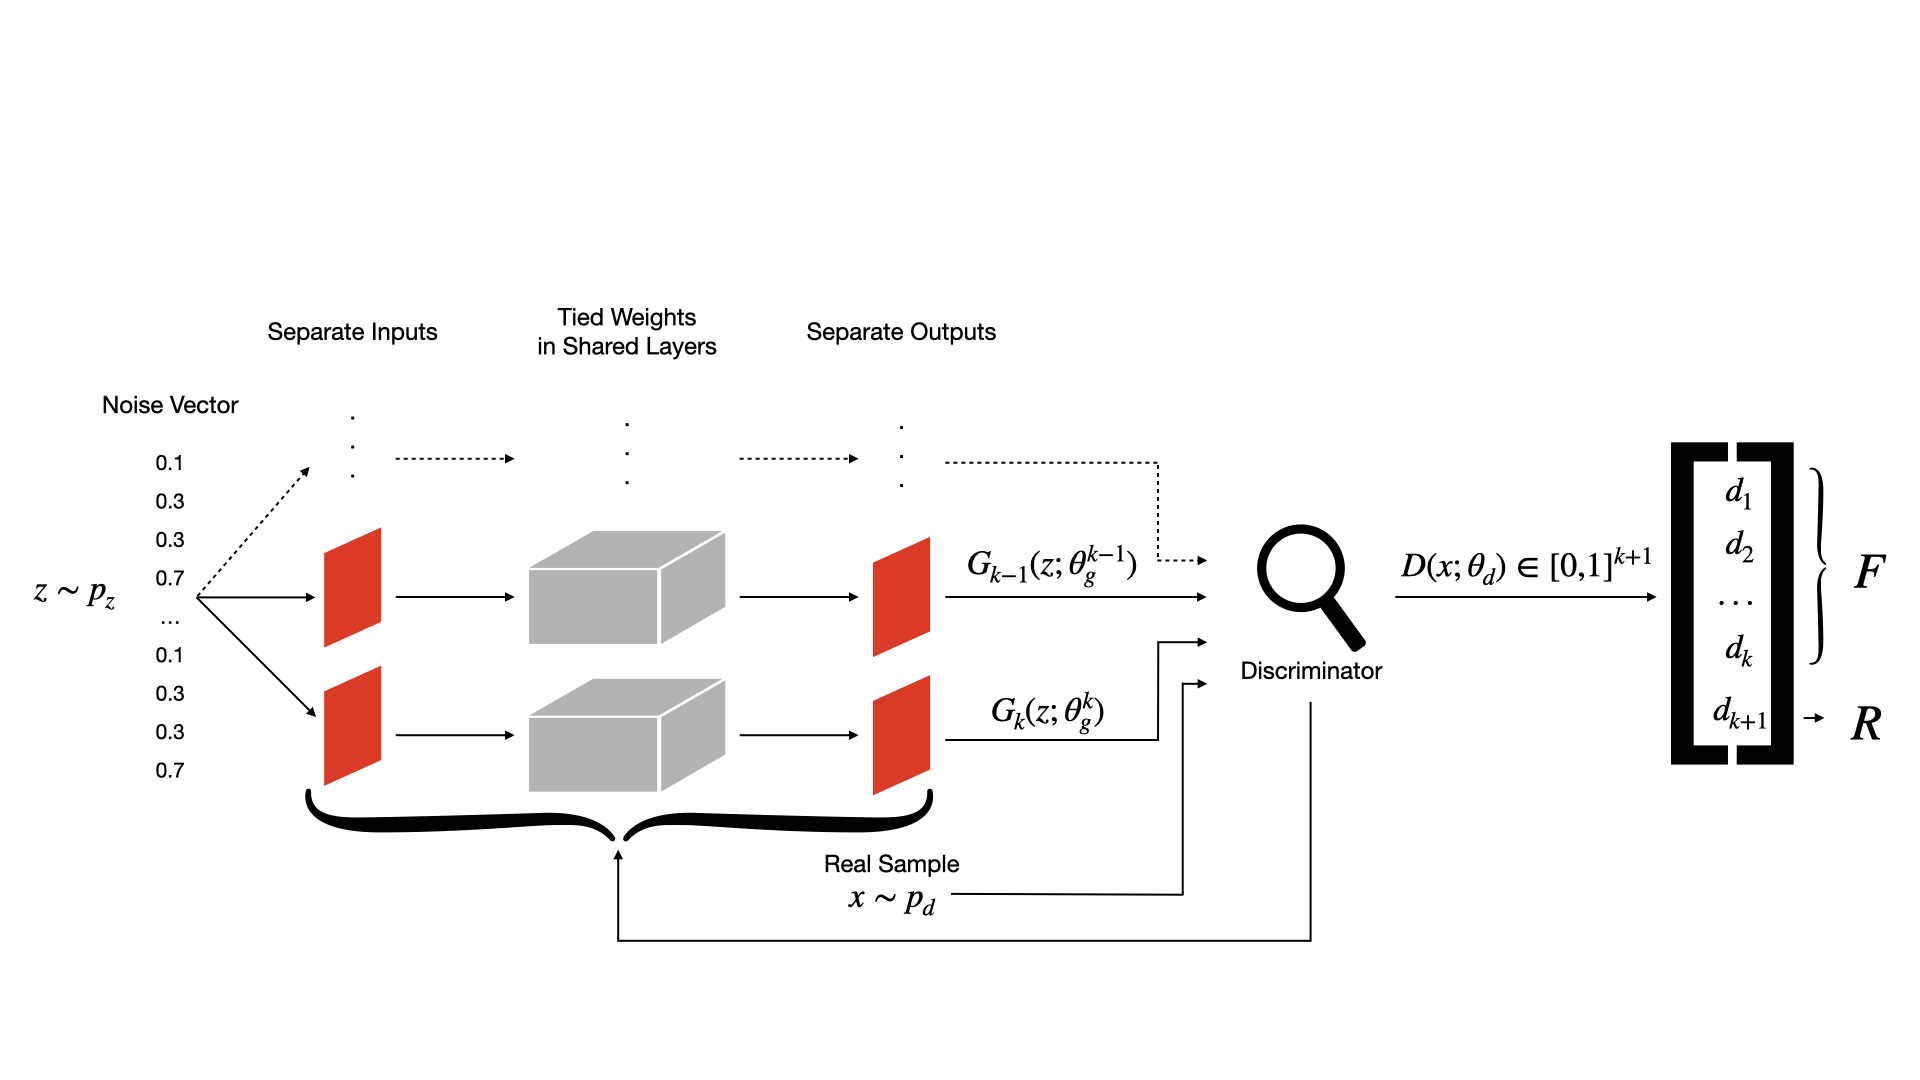
\includegraphics[width=.9\textwidth]{abb/arch_madgan.png}
    \caption{Visualization of the MADGAN architecture. The figure shows the \(k+1\) outputs of the discriminator and the \(k\) generators, with tied weights in the middle of the network.}
    \label{fig:figure_madgan_arch}
\end{figure}


\subsubsection{Mathematical Formulation}
\label{theoretical_madgan_math}
As afore mentioned, the MADGAN architecture employs multiple generators and one discriminator. The goal for the \(K\) generators is to generate samples from different high probability regions of the data \(P_{data}\). In order to guide the generators into their respective direction, the objective of the discriminator has been modified. The objective no longer only has to differentiate between real and fake images, but also identify the generator that produced a given fake sample. Intuitively, the discriminator thereby forces the generators into mostly disjoint regions within the real data distribution. Inspired by the formulation for the discriminator in the paper \textit{Improved Techniques for Training GANs} \cite{salimans2016improvedtechniquestraininggans}, their discriminator model produces a \((k+1)\)-dimensional output vector using the \textit{Softmax} activation function (\ref{theoretical_activations_softmax}), where \(k\) is the number of generators. The output at index \(k+1\) represents the probability that the given sample belongs to the real data distribution \(P_{\text{data}}\), while the entries at indices \(j \in \{1, \ldots, k\}\) represent the probabilities that the sample originates from each of the \(k\) generators. The above Figure \ref{fig:figure_madgan_arch} shows a visualization of the architecture. Thus, when learning the discriminators parameters \(\theta_d\), the cross-entropy between the softmax outputs and the \textit{Dirac delta distribution} (Ddd) \(\delta \in \{0, 1\}^{k+1}\) is optimized. Here, \(\delta \in \{0,1\}^{k+1}\) is a one-hot vector defined as:

\[
\delta(i) = 
\begin{cases}
1, & \text{if the sample originates from the } i\text{-th generator, at positions:} \quad i \in \{1, \ldots, k\} \\
1, & \text{if the sample originates from } P_{\text{data}} \text{ at positions:} \quad i = k+1 \\
\end{cases}
\]
Since one of the above cases must be fulfilled, every other index in the resulting vector must be $0$. This means exactly one entry of \(\delta\) is 1, indicating the source of the sample.
Following this definition, the Ddd \(\delta\) can be understood as a one-hot encoding indicating whether a given sample is real of, and if not, from which generator it originates \footnote{It is important to point out, that the Dirac delta distribution is actually continuous. Their usage of the Ddd reminds of the Kronecker delta function, which \( \delta(i,j) = 1 \text{ for } i=j; 0 \text{ for } i \ne j \).}. The objective function for the optimization of \(\theta_d\), with \(\theta_g\) frozen is therefore:

\begin{equation}
    \max\limits_{\theta_d}\mathbb{E}_{x \sim p} H(\delta, D(x; \theta_d))
\end{equation}.

\noindent
\(H(...)\) here represents the negative cross-entropy function. Important to point out here is that, \textit{Intuitively, in order to correctly identify the generator that produced a given fake sample, the discriminator must learn to push different generators towards different identifiable modes.} \cite{ghosh2018madgan}, page 4. Figure \ref{fig:figure_madgan_diverse_mode_push} shows a visualization of the generators being pushed to different modes. This is explicitly encouraged in the discriminators objective function. The objective for the generators however, remains semantically the same as in the vanilla GAN \ref{theory_gan_vanilla_formula}. The difference here is that the objective function is generalized with an indexing \(i\) for the number of generators. That is, for the \(i\)-th generator, the objective function is to minimize:

\begin{equation}
    \mathcal{L}_{Gen_i} = \mathbf{E}_{x \sim P_{data}} [ \log D(X; \theta_d) ] + \mathbf{E}_{z \sim P_{z}} \log (1-D_{k+1}(G_i(z; \theta_{g}^{i}); \theta_x))
\end{equation}

\noindent\textbf{Enforcing Diverse Modes:}
The multi-agent framework by Ghosh et al. introduces a mechanism for promoting mode diversity through multiple generators. The core idea is formalized in \textbf{Theorem 1} \cite{ghosh2018madgan} (page 2), which demonstrates that, given an optimal discriminator, the \(k\) generators collectively form a mixture model.

The objective function for the set of generators, which they collectively minimize, is defined as:

\begin{equation}
\label{eq:madgan_gen_loss_original}
\mathcal{L}_{Gen_{[0...k]}} = \mathbf{E}_{x \sim P_{data}} [ \log D_{k+1}(X) ] + \sum_{i=1}^{k}\mathbf{E}_{x \sim p_{g_i}} [\log (1-D_{k+1}(x))]
\end{equation}

When the discriminator \(D_{k+1}\) reaches its optimal state for a given set of generator distributions, its output \(D^*_{k+1}(x)\) allows the generator's objective function to be re-expressed in terms of divergences between probability distributions. While the explicit algebraic steps are omitted for brevity in the paper \cite{ghosh2018madgan}, this transformation converts the cross-entropy terms in Equation \ref{eq:madgan_gen_loss_original} into a form involving Kullback-Leibler (KL) divergences. This is a standard technique in GAN proofs, where the problem of distinguishing \textit{real} from \textit{fake} becomes one of minimizing the \textit{distance} between distributions.

Specifically, at equilibrium, the generator objective boils down to minimizing:

\begin{equation}
\label{eq:madgan_theorem1_simplified}
\text{KL} \left( p_{data}(x) \| p_{avg}(x) \right) + k \cdot \text{KL} \left( \frac{1}{k}\sum_{i=1}^k p_{g_i}(x) \middle\| p_{avg}(x) \right) - (k+1)\log(k+1) + k\log k
\end{equation}
where \(k\) is the number of generators and \(p_{avg}(x) = \frac{p_{data}(x) + \sum_{i=1}^k p_{g_i}(x)}{k+1}\).

The key to understanding the constant term \( -(k+1)\log(k+1) + k\log k \) lies in how this transformed objective achieves its global minimum. This minimum value is reached precisely when the real data distribution \(p_{data}\) is perfectly matched by the average of the generator distributions, i.e., \(p_{data} = \frac{1}{k}\sum_{i=1}^{k} p_{g_i}\).

\noindent
Under this optimal condition (\(p_{data} = \frac{1}{k}\sum_{i=1}^{k} p_{g_i}\)):
\begin{enumerate}
    \item The average distribution \(p_{avg}(x)\) simplifies to \(p_{data}(x)\), as \\\(p_{avg}(x) = \frac{p_{data}(x) + k \cdot p_{data}(x)}{k+1} = \frac{(k+1)p_{data}(x)}{k+1} = p_{data}(x)\).
    \item Consequently, both KL-divergence terms in Equation \ref{eq:madgan_theorem1_simplified} become zero, as \(\text{KL}(P||Q) = 0\) if and only if \(P=Q\).
    \begin{itemize}
        \item \(\text{KL}(p_{data}(x) \| p_{avg}(x)) = \text{KL}(p_{data}(x)|\| p_{data}(x)) = 0\)
        \item \(k \cdot \text{KL}\left(\frac{1}{k}\sum_{i=1}^k p_{g_i}(x) \| p_{avg}(x)\right) = k \cdot \text{KL}(p_{data}(x) \| p_{data}(x)) = 0\)
    \end{itemize}
\end{enumerate}


Thus, at this global optimum, the generator's objective value is simply the constant term: \( -(k+1)\log(k+1) + k\log k \). This constant represents the baseline value of the divergence when the distributions are perfectly aligned, arising from the inherent mathematical structure of the objective function transformation.

It's significant to note that, for \(k=1\) (the case with a single generator), substituting \(k=1\) into this expression yields \( -(1+1)\log(1+1) + 1\log 1 = -2\log 2 + 0 = -\log 4 \). This value perfectly aligns with the known optimal value of the generator objective for the vanilla GAN, which is rooted in the Jensen-Shannon divergence as shown by Goodfellow et al. \cite{goodfellow2014generativeadversarialnetworks}. This consistency reinforces the correctness of Theorem 1.

The exact formulation of their theorem, proof, and propositions can be found in Ghosh et al. \cite{ghosh2018madgan}, following formulas (3) through (9).

\begin{figure}[htbp]
    \centering
    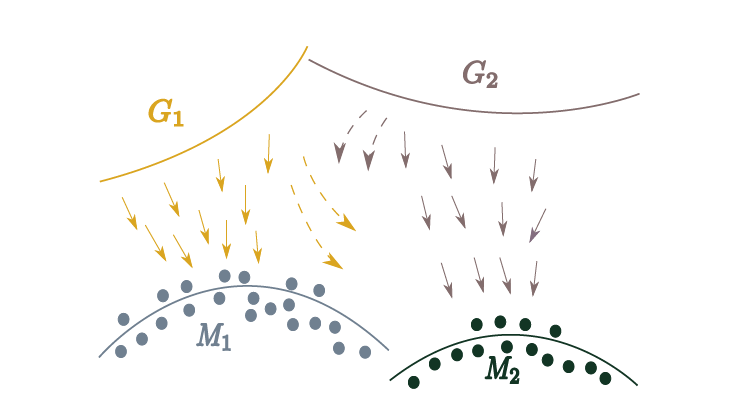
\includegraphics[width=.9\textwidth]{abb/madgan_diverse_mode_push.PNG}
    \caption{Figure taken from the original paper \cite{ghosh2018madgan}. The visualization shows how different generators \(G_ {1}\) and \(G_{2}\) are pushed to different modes \(M_{1}\) and \(M_{2}\), by the discriminator.}
    \label{fig:figure_madgan_diverse_mode_push}
\end{figure}

\subsubsection{Architectural Adjustments}
\label{theory_madgan_architecture}
The architectural changes can be summarized into three major changes applied to the vanilla GAN (\ref{theoretical_gan}) architecture:

\noindent\textbf{Multiple Generators:} The MADGAN architecture employs multiple generators instead of a single one. Following the intuition behind the adjusted discriminator objective, the outputs of the generators are distributed across different, mostly disjoint regions of the real data distribution.

\noindent\textbf{Modified Discriminator Objective:} The discriminator's last layer has an output of \(k + 1\), instead of \(1\)\footnote{Compared to the vanilla version of the architecture \ref{fig:figure_gan_arch}.} utilizing the softmax function \ref{theoretical_activations_softmax}. One output for every generator indicating whether an image originates from either one of the generator and one output implying if the discriminator came to the conclusion that the current image is fake or not. This encourages the discriminator to push the generators into identifiable distinct outputs (\ref{fig:figure_madgan_diverse_mode_push}).

\noindent\textbf{Parameter Sharing among Generators:} In the MADGAN architecture, the generators share all but the input and the final dense layer across the \(k\) generators. These shared layers function as a common feature extractor, reducing redundant computation in early feature extraction stages that capture high-frequency structures common to many datasets\footnote{For example, the first layers may detect horizontal and vertical edges, followed by corner detection, and so on.}. This setup is particularly recommended for single-view data, where the data distribution is more uniform. For multi-view data, however, parameter sharing is discouraged, as it may hinder each generator’s ability to learn mode-specific features.


% Define placeholder architectural functions
\newcommand{\definegenerator}{\texttt{define\_generator}}
\newcommand{\definediscriminator}{\texttt{define\_discriminator}}
% Define lambda symbol for diversity weight
\newcommand{\lambdadiv}{\lambda_{\text{div}}}
\subsection[Adapting MADGAN for Conditional Generation with Explicit Diversity - cMADGAN]{Adapting MADGAN for Conditional Generation with Explicit Diversity}
\label{theoretical_cmadgan}

The final goal of this research includes exploring methods for generating diverse samples in the mentioned datasets \ref{used_datasets} to be used for data augmentations. While the multi-agent framework by Ghosh et al. presents a potential approach, experiments revealed significant challenges in achieving stable training and satisfactory results in terms of image quality with the original method. Especially the CIFAR-10 dataset proved to be challenging, which is the only colored dataset used.

Consequently, an alternative framework, termed Conditional Multi-Agent Diverse GAN (cMADGAN), was conceptualized. The adjustment aims to retain the multi-generator diversity principle while simplifying the task of the discriminator. The discriminator model is rolled back to its original objective to differentiate between real and fake images. However, initial experiments indicated that this approach also faced convergence difficulties when applied to the original CIFAR-10 dataset. This specific is explained in more detail in the experiments section \ref{setup_cifar10_scope}.

The following sections detail the cMADGAN framework as implemented. This approach utilizes multiple generators ($G_1, \dots, G_K$), a single conditional discriminator ($D$) performing standard real/fake classification, and incorporates an explicit diversity loss between generator outputs alongside the adversarial objective.

\subsubsection{Mathematical Formulation}
\label{theoretical_cmadgan_math}

Let $z$ be a latent vector sampled from a prior distribution $p(z)$, typically a standard normal distribution. Let $c$ be the condition variable (e.g., class label) sampled from a distribution $p(c)$. The framework also employs $K$ generator networks $G_1, \dots, G_K$ and a single discriminator network $D$. Each generator $G_i$ maps an input pair $(z, c)$ to the data space, producing a fake sample $\hat{x}_i = G_i(z, c)$. The discriminator $D$ takes an input pair $(x, c)$ (where $x$ can be a real sample from the true data distribution $p_{\text{data}}(x|c)$ or a fake sample $\hat{x}_i$) and outputs a scalar probability estimating the likelihood that $x$ is real given the condition $c$.

The training involves optimizing two competing objectives, $\mathcal{L}_D$ for the discriminator and $\mathcal{L}_G$ for the generators:

\paragraph{Discriminator Loss:}
The discriminator is trained to distinguish real samples from fake samples generated by \textit{any} of the $K$ generators, given the condition $c$. Using the binary cross-entropy (BCE) loss, the objective is:
\begin{equation}
\label{eq:cmadgan_loss_d}
\begin{split}
\mathcal{L}_D = & - \mathbb{E}_{x \sim p_{\text{data}}(x|c), c \sim p(c)} [\log D(x, c)] \\
& - \frac{1}{K} \sum_{i=1}^{K} \mathbb{E}_{z \sim p(z), c \sim p(c)} [\log(1 - D(G_i(z, c), c))]
\end{split}
\end{equation}
This formulation averages the loss over the fake samples from all generators.

\paragraph{Generator Loss:}
The generators are trained collectively to fool the discriminator and simultaneously produce diverse outputs. The combined loss function for all generators includes an adversarial term and an explicit diversity term:
\begin{equation}
\label{eq:cmadgan_loss_g}
\mathcal{L}_G = \mathcal{L}_{\text{adv}} + \lambda_{div} \cdot \mathcal{L}_{\text{div}}
\end{equation}
where \(\lambda_{div}\) is a hyperparameter controlling the importance of the diversity component.

The components are defined as:
\begin{itemize}
    \item \textbf{Adversarial Loss ($\mathcal{L}_{\text{adv}}$):} Encourages generators to produce samples that the discriminator classifies as real. This is the sum of the non-saturating losses for each generator:
    \begin{equation}
    \label{eq:cmadgan_loss_g_adv}
    \mathcal{L}_{\text{adv}} = - \sum_{i=1}^{K} \mathbb{E}_{z \sim p(z), c \sim p(c)} [\log D(G_i(z, c), c)]
    \end{equation}

    \item \textbf{Diversity Loss ($\mathcal{L}_{\text{div}}$):} This term actively pushes the outputs of different generators apart. The goal during optimization ($\min \mathcal{L}_G$) is to maximize diversity. This is achieved by minimizing the negative cosine similarity. Cosine similarity is defined as:
    \begin{equation}
    \label{eq:cmadgan_cossim}
    \text{CosSim}(a, b) = \frac{\text{vec}(a) \cdot \text{vec}(b)}{\|\text{vec}(a)\|_2 \|\text{vec}(b)\|_2}
    \end{equation}
    where $\text{vec}(\cdot)$ denotes flattening the image tensor into a vector and $\|\cdot\|_2$ represents the \textit{L2 norm}, also known as the Euclidean norm of a vector. The diversity loss is the average pairwise negative cosine similarity, which the optimizer seeks to minimize:
    \begin{equation}
    \label{eq:cmadgan_loss_g_div}
    \mathcal{L}_{\text{div}} = -\frac{1}{N_p} \sum_{i=1}^{K} \sum_{j=i+1}^{K} \mathbb{E}_{z \sim p(z), c \sim p(c)} [\text{CosSim}(G_i(z, c), G_j(z, c))]
    \end{equation}
    where $N_p = K(K-1)/2$ is the number of unique generator pairs. Minimizing the combined $\mathcal{L}_G$ in Eq. \ref{eq:cmadgan_loss_g} thus encourages fooling the discriminator while explicitly promoting diversity between generator outputs.
\end{itemize}

\subsubsection{Architectural Adjustments}
\label{theory_cmadgan_architecture}

The cMADGAN architecture makes specific adjustments compared to both standard conditional GANs and the original MADGAN:

\begin{itemize}
    \item \textbf{Multiple Generators:}
    As the original MADGAN framework proposed, the cMADGAN employs $K$ distinct generator networks. As suggested in the original paper, the generators do not share their weights, due to the selection of datasets (cf. section 4.1 in \cite{ghosh2018madgan}). Each generator takes both the latent vector $z$ and the condition $c$ as input.
    \item \textbf{Conditional Discriminator:}
    Unlike the original MADGAN discriminator, the task of the cMADGAN discriminator performs the standard conditional GAN task \ref{theory_cgan_architecture}. $D$ receives an image $x$ (real or fake) and its corresponding condition $c$, and outputs a single probability indicating whether the image is real given the condition.
    \item \textbf{Conditioning Mechanism:} Class conditioning $c$ is integrated into both generator and discriminator networks.
        \begin{itemize}
            \item In the generators, an embedding of the condition $c$ is concatenated with the latent vector $z$ at the input layer before being processed by the main network layers (e.g., transposed convolutions).
            \item In the discriminator, the condition embedding is typically concatenated with intermediate feature maps before the final classification output, following common practices for conditional discriminators \cite{mirza2014conditionalgenerativeadversarialnets}.
        \end{itemize}
    \item \textbf{Explicit Diversity Enforcement:} Diversity is not solely an emergent property of competition but is explicitly encouraged via the $\mathcal{L}_{\text{div}}$ term in the generator objective (Eq. \ref{eq:cmadgan_loss_g}), directly penalizing high similarity between the outputs of different generators for the same input $(z, c)$.
\end{itemize}

The specific convolutional layers, normalization techniques, and activation functions within the generator and discriminator networks follow standard deep convolutional GAN (DCGAN) \cite{Radford2015DCGAN} principles and other relevant architectural patterns. This cMADGAN structure provides a framework for conditional generation that leverages multiple generators for diversity.


% ########################################################################################################
% # END: Generative Aderserial Networks
% ########################################################################################################


% ########################################################################################################
% # START: Image Scores
% ########################################################################################################

\subsection{Image Scores}\label{theoretical_image_scores}

To quantitatively evaluate the quality and diversity of images generated by generative models, several metrics have been proposed in the literature. These image scores aim to provide an objective measure to compare generative models independently of human evaluation. This section introduces widely-used metrics for evaluating generative models: \textit{Inception Score} (IS), \textit{Fréchet Inception Distance} (FID), and the underlying InceptionV3 model employed for these metrics.

\subsubsection[Inception Score - IS]{Inception Score}
The Inception Score (IS) \cite{salimans2016improvedtechniquestraininggans} is one of the earliest and most commonly used metrics for evaluating generative models, especially GANs. It leverages a pretrained InceptionV3 classifier to assess two main criteria of generated images:

\begin{itemize}
    \item \textbf{Image Quality (Clarity)}: Each generated image should be classified into a specific class with high confidence. This corresponds to a low-entropy conditional label distribution \( p(y|x) \).
    \item \textbf{Diversity}: Across the entire set of generated images, the distribution of predicted classes should be diverse and cover many labels. This corresponds to a high-entropy marginal label distribution \( p(y) \).
\end{itemize}

\noindent
Mathematically, the Inception Score is computed over a set of generated images \(x\) drawn from the generator's distribution \(p_g\):
\begin{equation}
IS = \exp \left( \mathbb{E}_{x \sim p_g} \left[ D_{\text{KL}}(p(y|x) \| p(y)) \right] \right)
\end{equation}
where \( D_{\text{KL}} \) denotes the Kullback-Leibler divergence between the conditional class distribution \(p(y|x)\) for a specific image \(x\) and the marginal class distribution \(p(y)\) estimated over all generated images. 

\noindent\textbf{Interpretation}:
A higher IS indicates that the model generates images that are confidently classified into diverse classes.

\noindent\textbf{Limitations of IS}:
\begin{itemize}
    \item Does not directly compare generated images with real images.
    \item Insensitive to intra-class diversity (e.g., generating only one type of dog within the dog class).
    \item Sensitive to the choice and specific training of the pretrained classifier.
\end{itemize}

\subsubsection[Fréchet Inception Distance - FID]{Fréchet Inception Distance}

The Fréchet Inception Distance (FID) \cite{heusel2018ganstrainedtimescaleupdate} improves upon IS by directly comparing the feature distributions of real and generated images. FID embeds both real (\(r\)) and generated (\(g\)) images into a lower-dimensional feature space using a pretrained \textit{InceptionV3} network (typically using the activations from the final average pooling layer, often referred to as 'pool3'). Each image is mapped to a fixed-length feature vector (embedding) consisting of all activation values from this layer. The embeddings across many images are then used to estimate two multivariate Gaussian distributions, one for real and one for generated data, by computing their empirical mean and covariance.


Let \( (\mu_r, \Sigma_r) \) and \( (\mu_g, \Sigma_g) \) denote the means and covariance matrices of the real and generated image Inception feature embeddings, respectively. The FID score is computed as the Fréchet distance (also known as Wasserstein-2 distance) between these two multivariate Gaussian distributions:
\begin{equation}
\text{FID} = \| \mu_r - \mu_g \|^2_2 + \text{Tr} \left( \Sigma_r + \Sigma_g - 2\left( \Sigma_r \Sigma_g \right)^{1/2} \right)
\end{equation}
where \( \|\cdot\|^2_2 \) is the squared \textit{L2 norm} (or Euclidean norm), \( \text{Tr}(\cdot) \) is the trace of a matrix, and \( \left( \Sigma_r \Sigma_g \right)^{1/2} \) denotes the **matrix square root of the matrix product** (i.e., standard matrix multiplication, not element-wise) between the two covariance matrices. The matrix square root \( A^{1/2} \) of a positive semi-definite matrix \( A \) is defined such that \( A^{1/2} A^{1/2} = A \).


\noindent\textbf{Interpretation}:
Lower FID indicates that the distribution of generated image features is more similar to the distribution of real image features, suggesting better quality and diversity. A score of 0 indicates identical distributions.

\noindent\textbf{Advantages over IS}:
\begin{itemize}
    \item Directly compares the generated image distribution to the real image distribution.
    \item More sensitive to intra-class mode collapse (lack of diversity within classes) as this affects \(\Sigma_g\).
    \item Generally found to correlate better with human judgment of image quality than IS.
\end{itemize}

\noindent\textbf{Limitations of FID}:
\begin{itemize}
    \item Assumes Gaussian distribution of features, which might be an approximation.
    \item Sensitive to the choice of feature extractor network and the specific layer used.
    \item Sensitive to both image quality (influencing feature representations) and diversity (influencing the mean and covariance of features).
    \item Requires a sufficiently large number of samples (both real and generated) for stable estimation of moments (\(\mu, \Sigma\)).
\end{itemize}

\subsubsection[InceptionV3 Model]{InceptionV3 for Image Evaluation}

Both IS and FID commonly rely on the InceptionV3 model~\cite{szegedy2016rethinking}, a deep convolutional neural network pretrained on the large-scale ImageNet dataset \cite{ImageNetDataset5206848}. The InceptionV3 network serves two primary roles in evaluating generative models:

\begin{enumerate}
    \item \textbf{Feature Extractor (for FID)}: Intermediate activations, typically from the final average pooling layer \textit{pool3}, are used as a semantic feature representation of the images. The statistics (mean and covariance) of these features are then compared between real and generated image sets.
    \item \textbf{Classifier (for IS)}: The output layer provides class probabilities for input images. These probabilities are used to calculate the entropy terms required for the Inception Score.
\end{enumerate}

\noindent\textbf{Properties of InceptionV3 relevant for image scoring}:
\begin{itemize}
    \item Trained on the diverse ImageNet dataset, providing a rich semantic feature space capable of capturing complex visual patterns.
    \item Uses fixed, non-trainable weights during evaluation, ensuring standardization and comparability of scores across different studies, provided the same implementation is used.
    \item The choice of layer for feature extraction (primarily for FID) impacts sensitivity; earlier layers capture lower-level features like texture, while later layers capture more abstract semantic information. The \textit{pool3} layer is commonly chosen as a balance.
\end{itemize}

\noindent\textbf{Limitations of using InceptionV3}:\label{theoretical_inception_model_limitaitions}
\begin{itemize}
    \item Domain Gap: The features learned on ImageNet (mostly natural images centered on objects) might not be optimally suited for evaluating images from significantly different domains, such as medical scans, satellite imagery, or abstract art.
    \item Sensitivity to ImageNet Classes: Performance, particularly for IS, can be less meaningful if the generated images depict objects or scenes vastly different from the $1 000$ ImageNet classes.
    \item Potential Bias: Potential biases present within the ImageNet dataset itself (e.g., representation bias) may be inherited by the features, potentially impacting evaluation fairness or relevance for specific target domains.
\end{itemize}


% ########################################################################################################
% # STOP: Image Scores
% ########################################################################################################

\newpage
